\documentclass[a4paper,11pt,oneside]{article}
\include{preambule}
\begin{document}

\begin{center}
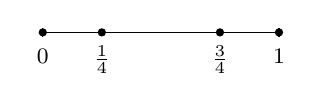
\begin{tikzpicture}[scale=3]
        \draw[line width=0.1mm] (0,0) -- (1,0);
            \foreach \x in {0,1} \draw[shift={(\x,0)},color=black] (0pt,0.5pt) -- (0pt,-0.5pt);
      \foreach \x in {1,3} \node at (\x/4,-0.115) {\footnotesize $\frac{\x}{4}$};
      \foreach \x in {0,1} \node at (\x,-0.1) {\footnotesize $\x$};
	\foreach \x in {0,1,3,4} \draw [fill] ({\x/4},0) circle (0.15mm);
      % \node at (-0.1,1) {\footnotesize $1$};
             \end{tikzpicture}
\end{center}

 \begin{center}
\begin{tikzpicture}
 \pgfmathsetmacro{\ray}{1.7}
  \pgfmathsetmacro{\lg}{3.3}
  \draw (-\lg,0)--(\lg+1,0) ;
   \draw (0,-0.08)--(0,0.08) ;
 \node at (-1.7,-0.3) {$\text{AC}$};
  \node at (2.3,-0.3) {$\text{DG}$};
    \node at (0,-0.4) {$R_a$};
    \node at (-\lg,-0.4) {$0$};
        \node at (-\lg,0) {\scriptsize $\bullet$};
 \end{tikzpicture}
\end{center}

\begin{center}
\begin{tikzpicture}[scale=0.85]
  \draw (0,0) -- (7,0);
  \end{tikzpicture}
\end{center}


\begin{center}
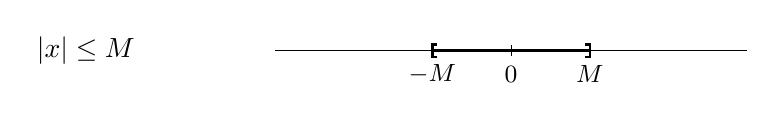
\begin{tikzpicture}[scale=1]
  \draw (-3,0) -- (3,0);
  \node at (-5.4,0) {$|x| \leq M$};
  \draw[shift={(0,0)},color=black] (0pt,2pt) -- (0pt,-2pt) ;
  \node at (0,-0.3) {\small $0$};
  \node at (1,-0.3) {\small $M$};
  \node at (-1,-0.3) {\small $-M$};
  \draw[line width=0.35mm]  (-1,0) -- (1,0) ;
   \pgfmathsetmacro{\haut}{0.08}
   \pgfmathsetmacro{\retour}{0.06}
  \draw[shift={(-1,0)},line width=0.3mm]  (\retour,-\haut) -- (0,-\haut) -- (0,\haut) -- (\retour,\haut) ;
  \draw[shift={(1,0)},line width=0.3mm]  (-\retour,-\haut) -- (0,-\haut) -- (0,\haut) -- (-\retour,\haut) ;
  \end{tikzpicture}
\end{center}

\begin{center}
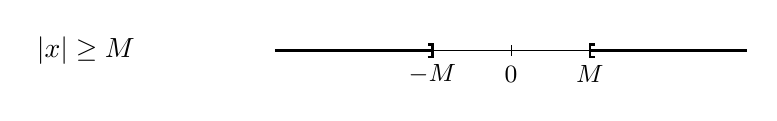
\begin{tikzpicture}[scale=1]
  \draw (-3,0) -- (3,0);
  \node at (-5.4,0) {$|x| \geq M$};
  \draw[shift={(0,0)},color=black] (0pt,2pt) -- (0pt,-2pt);
  \node at (0,-0.3) {\small $0$};
  \node at (1,-0.3) {\small $M$};
  \node at (-1,-0.3) {\small $-M$};
  \draw[line width=0.35mm]  (-3,0) -- (-1,0) ;
  \draw[line width=0.35mm]  (1,0) -- (3,0) ;
   \pgfmathsetmacro{\haut}{0.08}
   \pgfmathsetmacro{\retour}{0.06}
  \draw[shift={(-1,0)},line width=0.3mm]  (-\retour,-\haut) -- (0,-\haut) -- (0,\haut) -- (-\retour,\haut) ;
  \draw[shift={(1,0)},line width=0.3mm]  (\retour,-\haut) -- (0,-\haut) -- (0,\haut) -- (\retour,\haut) ;
  \end{tikzpicture}
\end{center}

\begin{center}

\begin{tikzpicture}[scale=1.2]
  \draw (-1,0) -- (4,0);
  \draw[shift={(0,0)},color=black] (0pt,2pt) -- (0pt,-2pt);
  \node at (0,-0.3) {\footnotesize $0$};
   \begin{scope}[shift={(0.2,0)}]
    \node at (0.414,-0.3) {\footnotesize $\sqrt{2}-1$};
    \node at (1.414,-0.3) {\footnotesize $\sqrt{2}$};
  \node at (2.414,-0.3) {\footnotesize $\sqrt{2}+1$};
  \draw[line width=0.35mm]  (0.414,0) -- (2.414,0) ;
  \pgfmathsetmacro{\haut}{0.08}
   \pgfmathsetmacro{\retour}{0.06}
  \draw[shift={(0.414,0)},line width=0.3mm]  (\retour,-\haut) -- (0,-\haut) -- (0,\haut) -- (\retour,\haut) ;
  \draw[shift={(2.414,0)},line width=0.3mm]  (-\retour,-\haut) -- (0,-\haut) -- (0,\haut) -- (-\retour,\haut) ;
   \draw[shift={(1.414,0)},color=black] (0pt,2pt) -- (0pt,-2pt);
   \end{scope}
  \end{tikzpicture}
\end{center}


\begin{center}
\begin{tikzpicture}[scale=1]
\pgfmathsetmacro{\xmin}{-3.5}
\pgfmathsetmacro{\xmax}{3.5}
\pgfmathsetmacro{\xa}{0.5}
\pgfmathsetmacro{\xb}{1.5}
\pgfmathsetmacro{\hauteur}{0.4}
\pgfmathsetmacro{\hauteurd}{\hauteur+0.3}
  \draw (\xmin,0) -- (\xmax,0);
  \draw[shift={(0,0)},color=black] (0pt,2pt) -- (0pt,-2pt) ;
  \node at (0,-0.3) {\small $\ell$};
  \draw[->,line width=0.28mm]  (\xb,\hauteur) -- (\xa,\hauteur) ;
  \node at ({(\xa+\xb)/2},\hauteurd) {\small $v_{n}$};
  \draw[->,line width=0.28mm]  (-\xb,\hauteur) -- (-\xa,\hauteur) ;
  \node at ({(-\xa-\xb)/2},\hauteurd) {\small $u_{n}$};
\end{tikzpicture}
\end{center}


\begin{center}
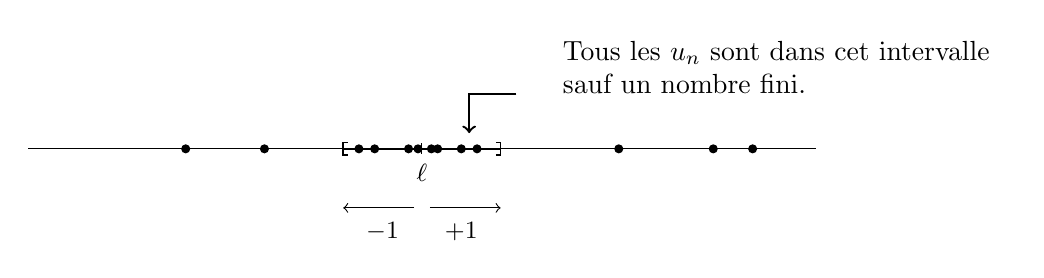
\begin{tikzpicture}[scale=1]
\pgfmathsetmacro{\xmin}{-5}
\pgfmathsetmacro{\xmax}{5}
\pgfmathsetmacro{\ext}{1}
  \draw (\xmin,0) -- (\xmax,0);
  \draw[shift={(0,0)},color=black] (0pt,2pt) -- (0pt,-2pt) ;
  \node at (0,-0.3) {\small $\ell$};
   \node at (\ext+3.5,1) {\begin{tabular}{l}
Tous les $u_n$ sont dans cet intervalle\\
sauf un nombre fini.
\end{tabular}};
\draw[->,line width=0.3mm]  (1.2*\ext,.7) -- (.6*\ext,.7) -- (.6*\ext,.2) ;
  \draw[line width=0.2mm]  (-\ext,0) -- (\ext,0) ;
   \pgfmathsetmacro{\haut}{0.08}
   \pgfmathsetmacro{\retour}{0.06}
  \draw[shift={(-\ext,0)},line width=0.2mm]  (\retour,-\haut) -- (0,-\haut) -- (0,\haut) -- (\retour,\haut) ;
  \draw[shift={(\ext,0)},line width=0.2mm]  (-\retour,-\haut) -- (0,-\haut) -- (0,\haut) -- (-\retour,\haut) ;
  \pgfmathsetmacro{\prof}{-0.75}
  \pgfmathsetmacro{\ecart}{0.1*\ext}
  \draw[->]  (\ecart,\prof) -- (\ext,.\prof) ;
  \node at (0.5*\ext,\prof-0.3) {\small $+1$};
  \draw[->]  (-\ecart,\prof) -- (-\ext,.\prof) ;
  \node at (-0.5*\ext,\prof-0.3) {\small $-1$};
  \foreach \x in {-3,-2,2.5,3.7,4.2} \draw [fill] (\x,0) circle (0.5 mm);
   \foreach \x in {-0.8,-0.6,0.12,0.2,0.7,-0.05,-0.17,0.5} \draw [fill] (\x,0) circle (0.5 mm);
\end{tikzpicture}
\end{center}


\begin{center}
\begin{tikzpicture}[scale=1]
\pgfmathsetmacro{\ext}{1.5}
  \draw (-5,0) -- (3,0);
  \draw[shift={(0,0)},color=black] (0pt,2pt) -- (0pt,-2pt) ;
    \draw[shift={(-\ext,0)},color=black] (0pt,2pt) -- (0pt,-2pt) ;
  \node at (0,-0.3) {\small $\la$};
  \node at (-\ext,-0.3) {\small $\la-\eps$};
  \node at (-1.2*\ext,.7) {$f(x_{0})$};
\draw[->,line width=0.3mm]  (-0.8*\ext,.7) -- (-.4*\ext,.7) -- (-.4*\ext,.2) ;
\draw[fill] (-.4*\ext,0) circle (0.5mm);
   \end{tikzpicture}
\end{center}


\begin{center}
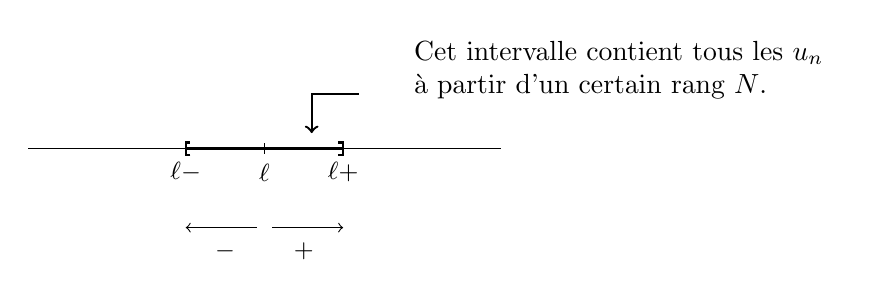
\begin{tikzpicture}[scale=1]
\pgfmathsetmacro{\ext}{1}
  \draw (-3,0) -- (3,0);
  \draw[shift={(0,0)},color=black] (0pt,2pt) -- (0pt,-2pt) ;
  \node at (0,-0.3) {\small $\ell$};
  \node at (\ext,-0.3) {\small $\ell+\eps$};
  \node at (-\ext,-0.3) {\small $\ell-\eps$};
  \node at (\ext+3.5,1) {\begin{tabular}{l}
Cet intervalle contient tous les $u_n$\\
à partir d'un certain rang $N$.
\end{tabular}};
\draw[->,line width=0.3mm]  (1.2*\ext,.7) -- (.6*\ext,.7) -- (.6*\ext,.2) ;
  \draw[line width=0.35mm]  (-\ext,0) -- (\ext,0) ;
   \pgfmathsetmacro{\haut}{0.08}
   \pgfmathsetmacro{\retour}{0.06}
  \draw[shift={(-\ext,0)},line width=0.3mm]  (\retour,-\haut) -- (0,-\haut) -- (0,\haut) -- (\retour,\haut) ;
  \draw[shift={(\ext,0)},line width=0.3mm]  (-\retour,-\haut) -- (0,-\haut) -- (0,\haut) -- (-\retour,\haut) ;
  \pgfmathsetmacro{\prof}{-1}
  \pgfmathsetmacro{\ecart}{0.1*\ext}
  \draw[->]  (\ecart,\prof) -- (\ext,.\prof) ;
  \node at (0.5*\ext,\prof-0.3) {\small $+\eps$};
  \draw[->]  (-\ecart,\prof) -- (-\ext,.\prof) ;
  \node at (-0.5*\ext,\prof-0.3) {\small $-\eps$};
\end{tikzpicture}
\end{center}


\begin{center}
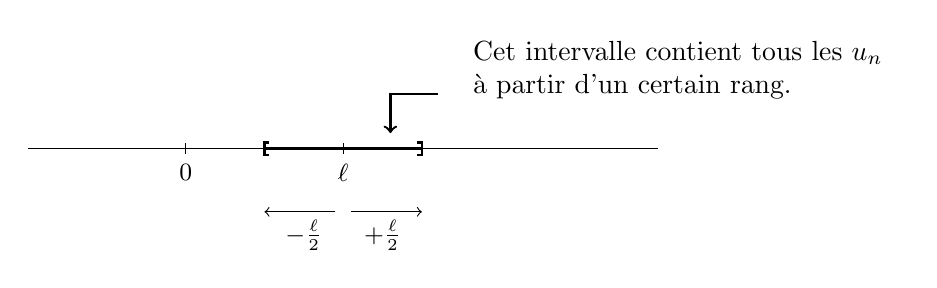
\begin{tikzpicture}[scale=1]
\pgfmathsetmacro{\ext}{1}
\pgfmathsetmacro{\xmin}{-4}
\pgfmathsetmacro{\xmax}{4}
  \draw (\xmin,0) -- (\xmax,0);
  \draw[shift={(0,0)},color=black] (0pt,2pt) -- (0pt,-2pt) ;
    \draw[shift={(-2,0)},color=black] (0pt,2pt) -- (0pt,-2pt) ;
  \node at (0,-0.3) {\small $\ell$};
   \node at (-2,-0.3) {\small $0$};
 % \node at (\ext,-0.3) {\small $\ell+\eps$};
  %\node at (-\ext,-0.3) {\small $\ell-\eps$};
  \node at (\ext+3.25,1) {\begin{tabular}{l}
Cet intervalle contient tous les $u_n$\\
à partir d'un certain rang.
\end{tabular}};
\draw[->,line width=0.3mm]  (1.2*\ext,.7) -- (.6*\ext,.7) -- (.6*\ext,.2) ;
  \draw[line width=0.35mm]  (-\ext,0) -- (\ext,0) ;
   \pgfmathsetmacro{\haut}{0.08}
   \pgfmathsetmacro{\retour}{0.06}
  \draw[shift={(-\ext,0)},line width=0.3mm]  (\retour,-\haut) -- (0,-\haut) -- (0,\haut) -- (\retour,\haut) ;
  \draw[shift={(\ext,0)},line width=0.3mm]  (-\retour,-\haut) -- (0,-\haut) -- (0,\haut) -- (-\retour,\haut) ;
  \pgfmathsetmacro{\prof}{-0.8}
  \pgfmathsetmacro{\ecart}{0.1*\ext}
  \draw[->]  (\ecart,\prof) -- (\ext,.\prof) ;
  \node at (0.5*\ext,\prof-0.3) {\small $+\frac{\ell}{2}$};
  \draw[->]  (-\ecart,\prof) -- (-\ext,.\prof) ;
  \node at (-0.5*\ext,\prof-0.3) {\small $-\frac{\ell}{2}$};
\end{tikzpicture}
\end{center}


\begin{center}
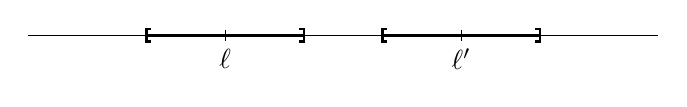
\begin{tikzpicture}[scale=1]
\pgfmathsetmacro{\xmin}{-4}
\pgfmathsetmacro{\xmax}{4}
\pgfmathsetmacro{\cun}{-1.5}
\pgfmathsetmacro{\cdeux}{1.5}
\pgfmathsetmacro{\ecartun}{1}
\pgfmathsetmacro{\ecartdeux}{\ecartun}
\pgfmathsetmacro{\xaun}{\cun-\ecartun}
\pgfmathsetmacro{\xbun}{\cun+\ecartun}
\pgfmathsetmacro{\xadeux}{\cdeux-\ecartdeux}
\pgfmathsetmacro{\xbdeux}{\cdeux+\ecartdeux}
\pgfmathsetmacro{\prof}{0.3}
  \draw (\xmin,0) -- (\xmax,0);
  \draw[shift={(\cun,0)},color=black] (0pt,2pt) -- (0pt,-2pt) ;
  \draw[shift={(\cdeux,0)},color=black] (0pt,2pt) -- (0pt,-2pt) ;
  \node at (\cun,-\prof) {$\ell$};
  \node at (\cdeux,-\prof) {$\ell'$};
   \pgfmathsetmacro{\haut}{0.08}
   \pgfmathsetmacro{\retour}{0.06}
 \draw[line width=0.35mm]  (\xaun,0) -- (\xbun,0) ;
  \draw[shift={(\xaun,0)},line width=0.3mm]  (\retour,-\haut) -- (0,-\haut) -- (0,\haut) -- (\retour,\haut) ;
  \draw[shift={(\xbun,0)},line width=0.3mm]  (-\retour,-\haut) -- (0,-\haut) -- (0,\haut) -- (-\retour,\haut) ;
 \draw[line width=0.35mm]  (\xadeux,0) -- (\xbdeux,0) ;
  \draw[shift={(\xadeux,0)},line width=0.3mm]  (\retour,-\haut) -- (0,-\haut) -- (0,\haut) -- (\retour,\haut) ;
  \draw[shift={(\xbdeux,0)},line width=0.3mm]  (-\retour,-\haut) -- (0,-\haut) -- (0,\haut) -- (-\retour,\haut) ;
    \end{tikzpicture}
\end{center}


\begin{center}
\begin{tikzpicture}[scale=1]
\pgfmathsetmacro{\xmin}{-4}
\pgfmathsetmacro{\xmax}{7}
\pgfmathsetmacro{\xa}{-1.2}
\pgfmathsetmacro{\xb}{2.8}
\pgfmathsetmacro{\epssillon}{0.65}
  \draw (\xmin,0) -- (\xmax,0);
  \draw[shift={(0,0)},color=black] (0pt,2pt) -- (0pt,-2pt) ;
  \draw[shift={(\epssillon,0)},color=black] (0pt,2pt) -- (0pt,-2pt) ;
  \draw[shift={(-\epssillon,0)},color=black] (0pt,2pt) -- (0pt,-2pt) ;
  \node at (0,-0.3) {\small $\ell$};
   \node at (\xa,-0.3) {\small $a$};
   \node at (\xb,-0.3) {\small $b$};
    \draw[line width=0.35mm]  (\xa,0) -- (\xb,0) ;
   \pgfmathsetmacro{\haut}{0.08}
   \pgfmathsetmacro{\retour}{0.06}
  \draw[shift={(\xb,0)},line width=0.3mm]  (\retour,-\haut) -- (0,-\haut) -- (0,\haut) -- (\retour,\haut) ;
  \draw[shift={(\xa,0)},line width=0.3mm]  (-\retour,-\haut) -- (0,-\haut) -- (0,\haut) -- (-\retour,\haut) ;
  \pgfmathsetmacro{\hauteur}{0.2}
  \draw[<->]  (0,\hauteur) -- (\epssillon,\hauteur) ;
  \draw[<->]  (0,\hauteur) -- (-\epssillon,\hauteur) ;
  \node at (0.5*\epssillon,2*\hauteur) {\small $\eps$};
  \node at (-0.5*\epssillon,2*\hauteur) {\small $\eps$};
  \end{tikzpicture}
\end{center}




\begin{center}
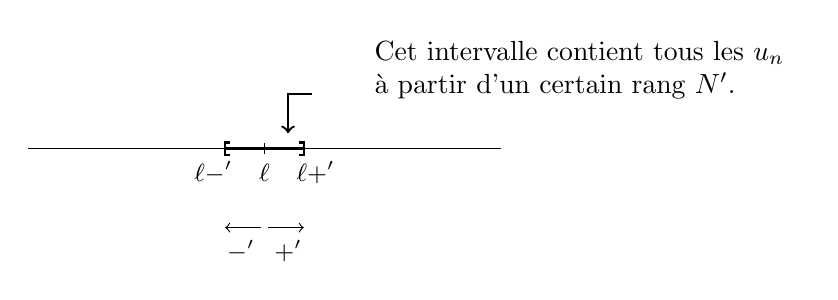
\begin{tikzpicture}[scale=1]
\pgfmathsetmacro{\ext}{0.5}
  \draw (-3,0) -- (3,0);
  \draw[shift={(0,0)},color=black] (0pt,2pt) -- (0pt,-2pt) ;
  \node at (0,-0.3) {\small $\ell$};
  \node at (1.3*\ext,-0.3) {\small $\ell+\eps'$};
  \node at (-1.3*\ext,-0.3) {\small $\ell-\eps'$};
  \node at (\ext+3.5,1) {\begin{tabular}{l}
Cet intervalle contient tous les $u_n$\\
à partir d'un certain rang $N'$.
\end{tabular}};
\draw[->,line width=0.3mm]  (1.2*\ext,.7) -- (.6*\ext,.7) -- (.6*\ext,.2) ;
  \draw[line width=0.35mm]  (-\ext,0) -- (\ext,0) ;
   \pgfmathsetmacro{\haut}{0.08}
   \pgfmathsetmacro{\retour}{0.06}
  \draw[shift={(-\ext,0)},line width=0.3mm]  (\retour,-\haut) -- (0,-\haut) -- (0,\haut) -- (\retour,\haut) ;
  \draw[shift={(\ext,0)},line width=0.3mm]  (-\retour,-\haut) -- (0,-\haut) -- (0,\haut) -- (-\retour,\haut) ;
  \pgfmathsetmacro{\prof}{-1}
  \pgfmathsetmacro{\ecart}{0.1*\ext}
  \draw[->]  (\ecart,\prof) -- (\ext,.\prof) ;
  \node at (0.6*\ext,\prof-0.3) {\small $+\eps'$};
  \draw[->]  (-\ecart,\prof) -- (-\ext,.\prof) ;
  \node at (-0.6*\ext,\prof-0.3) {\small $-\eps'$};
\end{tikzpicture}
\end{center}


\begin{center}
\begin{tikzpicture}[scale=1]
\pgfmathsetmacro{\xmin}{-4}
\pgfmathsetmacro{\xmax}{4}
 \pgfmathsetmacro{\haut}{0.08}
   \pgfmathsetmacro{\retour}{0.06}
\node at (-6,0) {$I_{0}$};
\node at (-6,-2) {$I_{1}$};
\node at (-6,-4) {$I_{2}$};
\node at (-6,-6) {$I_{4}$};
\node at (-6,-8) {$I_{6}$};
\foreach \h in {0,...,4} {
\draw (\xmin,-2*\h) -- (\xmax,-2*\h);
 \draw[shift={(\xmin,-2*\h)}]  (\retour,-\haut) -- (0,-\haut) -- (0,\haut) -- (\retour,\haut) ;
  \draw[shift={(\xmax,-2*\h)}]  (-\retour,-\haut) -- (0,-\haut) -- (0,\haut) -- (-\retour,\haut) ;
}
\foreach \x/\y/\h in {-4/4/0,-4/0/-2,-2/0/-4,-1/0/-6,-1/-0.5/-8} {
 \draw[line width=0.35mm]  (\x,\h) -- (\y,\h) ;
 \draw[shift={(\x,\h)},line width=0.3mm]  (\retour,-\haut) -- (0,-\haut) -- (0,\haut) -- (\retour,\haut) ;
  \draw[shift={(\y,\h)},line width=0.3mm]  (-\retour,-\haut) -- (0,-\haut) -- (0,\haut) -- (-\retour,\haut) ;
   }
   \pgfmathsetmacro{\prof}{0.35}
   \pgfmathsetmacro{\profd}{0.3975}
   \node at (-4,-\profd) {$a$};
   \node at (4,-\prof) {$b$};
    \node at (-4,-2-\profd) {$a_{1}$};
   \node at (0,-2-\prof) {$b_{1}$};
    \node at (-2,-4-\profd) {$a_{2}$};
   \node at (0,-4-\prof) {$b_{2}$};
    \node at (-1,-6-\profd) {$a_{3}$};
   \node at (0,-6-\prof) {$b_{3}$};
    \node at (-1,-8-\profd) {$a_{4}$};
   \node at (-0.5,-8-\prof) {$b_{4}$};

    \end{tikzpicture}
\end{center}



\begin{center}
\begin{tikzpicture}[scale=1]
\pgfmathsetmacro{\ext}{0.35}
  \draw (-3,0) -- (3,0);
  \draw[shift={(0,0)},color=black] (0pt,2pt) -- (0pt,-2pt) ;
  \node at (0,-0.3) {\small $\ell$};
  \node at (2*\ext,-0.3) {\small $\ell+\eps''$};
  \node at (-2*\ext,-0.3) {\small $\ell-\eps''$};
    \draw[line width=0.35mm]  (-\ext,0) -- (\ext,0) ;
   \pgfmathsetmacro{\haut}{0.08}
   \pgfmathsetmacro{\retour}{0.06}
  \draw[shift={(-\ext,0)},line width=0.3mm]  (\retour,-\haut) -- (0,-\haut) -- (0,\haut) -- (\retour,\haut) ;
  \draw[shift={(\ext,0)},line width=0.3mm]  (-\retour,-\haut) -- (0,-\haut) -- (0,\haut) -- (-\retour,\haut) ;
  \pgfmathsetmacro{\prof}{-1}
  \pgfmathsetmacro{\ecart}{0.1*\ext}
  \draw[->]  (\ecart,\prof) -- (\ext,.\prof) ;
  \node at (0.95*\ext,\prof-0.3) {\small $+\eps''$};
  \draw[->]  (-\ecart,\prof) -- (-\ext,.\prof) ;
  \node at (-0.95*\ext,\prof-0.3) {\small $-\eps''$};
\end{tikzpicture}
\end{center}

\begin{center}
\begin{tikzpicture}[scale=1]
\pgfmathsetmacro{\ext}{1}
\pgfmathsetmacro{\prof}{0.4}
  \draw (-3,0) -- (3,0);
  \draw[shift={(0,0)},color=black] (0pt,2pt) -- (0pt,-2pt) ;
  \node at (0,-\prof) {\small $\la$};
  \node at (1.3*\ext,-\prof) {\small $\la+\eps$};
  \node at (-1.3*\ext,-\prof) {\small $\la-\eps$};
  \node at (-1.3,0.75) {$u_{N}$};
\draw[->,line width=0.3mm]  (-1,0.7) -- (-0.6,0.7) -- (-0.6,0.2) ;
  \draw[line width=0.35mm]  (-\ext,0) -- (\ext,0) ;
   \pgfmathsetmacro{\haut}{0.08}
   \pgfmathsetmacro{\retour}{0.06}
  \draw[shift={(-\ext,0)},line width=0.3mm]  (\retour,-\haut) -- (0,-\haut) -- (0,\haut) -- (\retour,\haut) ;
  \draw[shift={(\ext,0)},line width=0.3mm]  (-\retour,-\haut) -- (0,-\haut) -- (0,\haut) -- (-\retour,\haut) ;
  \draw [fill] (-0.6,0) circle (0.5 mm);
  \end{tikzpicture}
\end{center}



\begin{center}
\begin{tikzpicture}[scale=1]
\pgfmathsetmacro{\xmin}{-4}
\pgfmathsetmacro{\xmax}{4}
\pgfmathsetmacro{\ext}{1.65}
  \draw (\xmin,0) -- (\xmax,0);
  \draw[shift={(0,0)},color=black] (0pt,2pt) -- (0pt,-2pt) ;
  \node at (0,-0.3) {\small $\ell$};
   \node at (\ext,-0.3) {\small $\ell+\eps$};
  \node at (-\ext,-0.3) {\small $\ell-\eps$};
 \draw[line width=0.3mm]  (-\ext,0) -- (\ext,0) ;
   \pgfmathsetmacro{\haut}{0.08}
   \pgfmathsetmacro{\retour}{0.06}
  \draw[shift={(-\ext,0)},line width=0.3mm]  (\retour,-\haut) -- (0,-\haut) -- (0,\haut) -- (\retour,\haut) ;
  \draw[shift={(\ext,0)},line width=0.3mm]  (-\retour,-\haut) -- (0,-\haut) -- (0,\haut) -- (-\retour,\haut) ;
  \pgfmathsetmacro{\prof}{-0.75}
  \pgfmathsetmacro{\ecart}{0.1*\ext}
  \pgfmathsetmacro{\xu}{0.5}
  \pgfmathsetmacro{\xv}{1.2}
    \foreach \x in {\xu,\xv} \draw [fill] (\x,0) circle (0.5 mm);
    \pgfmathsetmacro{\hauteur}{0.3}
    \node at (\xu,\hauteur) {\small $v_n$};
    \node at (\xv,\hauteur) {\small $w_n$};
\end{tikzpicture}
\end{center}


\begin{center}
\begin{tikzpicture}[scale=1]
  \draw (0,0) -- (7,0);
   \foreach \x in { 1 ,... , 6 }{\node at (\x,0) {\textbullet};
   \node at (\x,-0.3) {\footnotesize $\x$};
   };
   \draw[->,line width=0.25mm]  (3.5,-1.5) -- (3.5,0) ;
  \end{tikzpicture}
\end{center}

\begin{center}
\begin{tikzpicture}[scale=1]
  \draw (0.3,0) -- (11.7,0);
   \foreach \x in {1,...,11} \node at ({\x},0) {\textbullet};
  \node at (7.6,-0.25) {\footnotesize $a$};
   \node at (7,0.3) {\footnotesize $\pe{a}$};
   \node at (7.6,0) {\footnotesize $\times$};
    \node at (3.5,1) {$\zz$};
  \end{tikzpicture}
\end{center}


\begin{center}
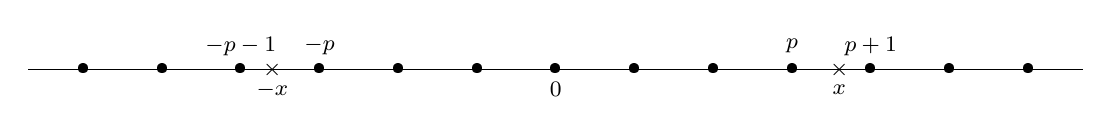
\begin{tikzpicture}[scale=1]
  \draw (-6.7,0) -- (6.7,0);
   \foreach \x in {-6,...,6} \node at ({\x},0) {\textbullet};
    \node at (0,-0.25) {\footnotesize $0$};
  \node at (3.6,-0.25) {\footnotesize $x$};
    \node at (-3.6,-0.25) {\footnotesize $-x$};
   \node at (3,0.3) {\footnotesize $p$};
   \node at (4,0.3) {\footnotesize $p+1$};
   \node at (-3,0.3) {\footnotesize $-p$};
   \node at (-4,0.3) {\footnotesize $-p-1$};
   \node at (3.6,0) {\footnotesize $\times$};
   \node at (-3.6,0) {\footnotesize $\times$};
  \end{tikzpicture}
\end{center}

\begin{center}
\begin{tikzpicture}[scale=1]
\pgfmathsetmacro{\xmin}{-6}
\pgfmathsetmacro{\xmax}{6}
  \draw (\xmin,0) -- (\xmax,0);
\pgfmathsetmacro{\xa}{0}
\pgfmathsetmacro{\xb}{2}  
  \draw[shift={(\xa,0)},color=black] (0pt,2pt) -- (0pt,-2pt) ;
   \draw[shift={(\xb,0)},color=black] (0pt,2pt) -- (0pt,-2pt) ;
  \node at (\xa,-0.3) {\small $\la$};
  \node at (\xb,-0.3) {\small $M$};
   \foreach \x in {-2,-1,-0.6666667,-0.5,-0.4,-0.33333,-0.28571,-0.25,-0.2222222,-0.2} \draw [fill] (\x,0) circle (0.5 mm);
    \foreach \x in {-0.18182,-0.16666667,-0.15385,-0.14286,-0.1333333,-0.125,-0.11765,-0.111111,-0.10526,-0.1} \draw [fill] (\x,0) circle (0.5 mm);
     \foreach \x in {-0.09524,-0.09091,-0.08696,-0.083333,-0.08,-0.07692,-0.07407,-0.07143,-0.06897,-0.0666667} \draw [fill] (\x,0) circle (0.5 mm);
  \end{tikzpicture}
\end{center}


\begin{center}
\begin{tikzpicture}[scale=2]
  \draw[line width=0.1mm] (-3,0) -- (3,0);
  \foreach \x in {-1,0,1} \draw[shift={(\x,0)},color=black] (0,0.05) -- (0,-0.05);
  \foreach \n in { 1 ,... , 7 } \node at ({1+1/(2*\n)},0) {\footnotesize \textbullet};
  \foreach \n in { 0 ,... , 7 } \node at ({-1+1/(4*\n+1)},0) {\footnotesize \textbullet};
   \foreach \n in { 1 ,... , 4 } \node at ({1+1/(8*\n)},0) {\footnotesize \textbullet};
  \foreach \n in { 0 ,... , 2 } \node at ({-1+1/(8*\n+1)},0) {\footnotesize \textbullet};
  \node at (0,-0.2) {\small $0$};
  \node at (1,-0.2) {\small $1$};
  \node at (-1,-0.2) {\small $-1$};
    \end{tikzpicture}
\end{center}


\begin{center}
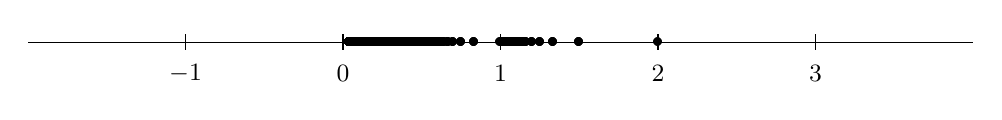
\begin{tikzpicture}[scale=2]
  \draw[line width=0.1mm] (-2,0) -- (4,0);
  \foreach \x in {-1,0,1,2,3} \draw[shift={(\x,0)},color=black] (0,0.05) -- (0,-0.05);
  \foreach \n in { 1 ,... , 50 } \foreach \p in { 1 ,... , 50 } \node at ({1/(\p)+1/(\n)},0) {\footnotesize \textbullet};
   \node at (0,-0.2) {\small $0$};
  \node at (1,-0.2) {\small $1$};
  \node at (2,-0.2) {\small $2$};
  \node at (3,-0.2) {\small $3$};
  \node at (-1,-0.2) {\small $-1$};
    \end{tikzpicture}
\end{center}


\begin{center}
\begin{tikzpicture}[scale=1]
  \draw[line width=0.1mm] (-6,0) -- (6,0);
  \foreach \x in {-3,-2.6,2.6,3} \draw[shift={(\x,0)},color=black] (0,0.05) -- (0,-0.05);
  \foreach \x in {-2.85,2.75 }\node at (\x,0) {\footnotesize \textbullet};
   \node at (-3,0.3) {\small $\alp$};
   \node at (3,0.3) {\small $\beta$};
    \draw[<->,line width=0.1mm] (-2.85,-0.5) -- (2.75,-0.5);
      \end{tikzpicture}
\end{center}

\begin{center}
\begin{tikzpicture}[scale=0.45]
  \pgfmathsetmacro{\lgun}{1}
   \pgfmathsetmacro{\lgmax}{28}
    \pgfmathsetmacro{\lgmaxmu}{\lgmax-1}
  \pgfmathsetmacro{\hauteur}{-0.7}
  \pgfmathsetmacro{\pointa}{22}
  \pgfmathsetmacro{\pointb}{5}
  \pgfmathsetmacro{\ecartfleche}{0.5}
  \pgfmathsetmacro{\hauteurfleche}{0.5}
  \pgfmathsetmacro{\pointr}{14.6}
  \draw[line width=0.1mm] (0,0) -- (\lgmax,0);
   \foreach \x in {0,...,\lgmaxmu} \draw[shift={(\lgun*\x,0)},color=black] (0,0.12) -- (0,-0.12);
   \foreach \x in {0,1,2} \node at (\x,\hauteur) {$\x$};
    \foreach \x in {0,...,5} \draw[fill] (\x*\pointb,0) circle (0.8 mm);
    \node at (\pointa,\hauteur) {\small $a$};
    \node at (\pointb,\hauteur) {\small $b$};
    \node at (2*\pointb,\hauteur) {\small $2b$};
    \node at (4*\pointb,\hauteur) {\small $qb$};
    \draw[->] (20,\hauteurfleche) -- (22,\hauteurfleche);
    \node at (21,\hauteurfleche+\ecartfleche) {\small $+r$};
    \end{tikzpicture}
\end{center}

\begin{center}
\begin{tikzpicture}[scale=1.15]
  \pgfmathsetmacro{\nmin}{-5}
    \pgfmathsetmacro{\nmax}{5}
  \pgfmathsetmacro{\xmin}{\nmin-0.5}
   \pgfmathsetmacro{\xmax}{\nmax+0.5}
  \pgfmathsetmacro{\hauteur}{-0.3}
  \pgfmathsetmacro{\pointa}{3.6}
  \pgfmathsetmacro{\pointqb}{3}
  \pgfmathsetmacro{\pointr}{0.5*\pointqb+0.5*\pointa}
  \pgfmathsetmacro{\ecartfleche}{0.3}
  \pgfmathsetmacro{\hauteurfleche}{0.3}
  \draw[line width=0.1mm] (\xmin,0) -- (\xmax,0);
   \foreach \x in {\nmin,...,\nmax} \draw[fill] (\x,0) circle (0.45 mm);
   \foreach \x in {\pointa,-\pointa} \draw (\x,0.06) -- (\x,-0.06);
   \node at (0,\hauteur) {\footnotesize  $0$};
    \node at (\pointa,\hauteur) {\footnotesize  $-a$};
        \node at (-\pointa,\hauteur) {\footnotesize  $a$};
    \node at (\pointqb,\hauteur) {\footnotesize $qb$};
    \node at (-\pointqb,\hauteur) {\footnotesize  $-qb$};
    \draw[->] (\pointqb,\hauteurfleche) -- (\pointa,\hauteurfleche);
    \node at (\pointr,\hauteurfleche+\ecartfleche) {\footnotesize $+r$};
    \draw[->] (-\pointqb,\hauteurfleche) -- (-\pointa,\hauteurfleche);
    \node at (-\pointr,\hauteurfleche+\ecartfleche) {\footnotesize $-r$};
\end{tikzpicture}
\end{center}

\begin{center}
\begin{tikzpicture}[scale=1.15]
  \pgfmathsetmacro{\nmin}{-5}
    \pgfmathsetmacro{\nmax}{5}
  \pgfmathsetmacro{\xmin}{\nmin-0.5}
   \pgfmathsetmacro{\xmax}{\nmax+0.5}
  \pgfmathsetmacro{\hauteur}{-0.3}
  \pgfmathsetmacro{\pointa}{3.6}
  \pgfmathsetmacro{\pointqb}{3}
   \pgfmathsetmacro{\pointqbp}{-\pointqb-1}
  \pgfmathsetmacro{\pointr}{0.5*\pointqb+0.5*\pointa}
   \pgfmathsetmacro{\pointrp}{0.5*\pointqbp-0.5*\pointa}
  \pgfmathsetmacro{\ecartfleche}{0.3}
  \pgfmathsetmacro{\hauteurfleche}{0.3}
  \draw[line width=0.1mm] (\xmin,0) -- (\xmax,0);
   \foreach \x in {\nmin,...,\nmax} \draw[fill] (\x,0) circle (0.45 mm);
   \foreach \x in {-\pointa} \draw (\x,0.06) -- (\x,-0.06);
   \node at (0,\hauteur) {\footnotesize  $0$};
     \node at (0.05-\pointa,\hauteur) {\footnotesize  $a$};
    \node at (\pointqbp-0.05,\hauteur) {\footnotesize  $q'b$};
    \draw[->] (\pointqbp,\hauteurfleche) -- (-\pointa,\hauteurfleche);
    \node at (\pointrp,\hauteurfleche+\ecartfleche) {\footnotesize $+r'$};
\end{tikzpicture}
\end{center}




\begin{center}
\begin{tikzpicture}[scale=0.6]
  \pgfmathsetmacro{\unsurq}{1}
  \pgfmathsetmacro{\hauteur}{-0.7}
  \pgfmathsetmacro{\pointa}{14}
  \pgfmathsetmacro{\pointb}{16}
  \pgfmathsetmacro{\ecartfleche}{0.05}
  \pgfmathsetmacro{\hauteurfleche}{0.35}
  \pgfmathsetmacro{\pointr}{14.6}
  \draw[line width=0.1mm] (-2,0) -- (20,0);
   \foreach \x in {0,1,2,3} \draw[shift={(\unsurq*\x,0)},color=black] (0,0.12) -- (0,-0.12);
  \node at (0,\hauteur) {\small $0$};
   \foreach \x in {1,2,3} \node at (\x,\hauteur) {$\frac{\x}{q}$};
   \node at (14.6,\hauteur) {$\frac{n}{q}$};
    \node at (\pointa,\hauteur) {\small $a$};
    \node at (\pointb,\hauteur) {\small $b$};
    \foreach \x in {0,1,2,3}  \draw [->] (\x+\ecartfleche,0.35) to[bend left] (\x+1-\ecartfleche,0.35);
    \node at (3.5,1) {$+\frac{1}{q}$};
    \node at (6,0.35) {\ldots};
    \point{(\pointr,0)}{0.6};
    \draw [->] (\pointr-\ecartfleche-1,\hauteurfleche) to[bend left] (\pointr-\ecartfleche,\hauteurfleche);
\pgfmathsetmacro{\haut}{0.15}
   \pgfmathsetmacro{\retour}{0.12}
  \draw[shift={(\pointa,0)},line width=0.3mm]  (-\retour,-\haut) -- (0,-\haut) -- (0,\haut) -- (-\retour,\haut) ;
  \draw[shift={(\pointb,0)},line width=0.3mm]  (\retour,-\haut) -- (0,-\haut) -- (0,\haut) -- (\retour,\haut) ;
\end{tikzpicture}
\end{center}

\begin{center}
\begin{tikzpicture}[scale=0.6]
  \pgfmathsetmacro{\unsurq}{1}
  \pgfmathsetmacro{\hauteur}{-0.7}
  \pgfmathsetmacro{\pointa}{14}
  \pgfmathsetmacro{\pointb}{16}
  \pgfmathsetmacro{\ecartfleche}{0.05}
  \pgfmathsetmacro{\hauteurfleche}{0.35}
  \pgfmathsetmacro{\pointr}{14.6}
  \draw[line width=0.1mm] (-2,0) -- (20,0);
   \foreach \x in {0,1,2,3} \draw[shift={(\unsurq*\x,0)},color=black] (0,0.12) -- (0,-0.12);
  \node at (0,\hauteur) {\small $0$};
   \foreach \x in {1,2,3} \node at (\x,\hauteur) {\scriptsize $\frac{\x}{10^{n}}$};
   \node at (14.6,\hauteur) {\scriptsize $\frac{k}{10^{n}}$};
    \node at (\pointa,\hauteur) {\small $a$};
    \node at (\pointb,\hauteur) {\small $b$};
    \foreach \x in {0,1,2,3}  \draw [->] (\x+\ecartfleche,0.35) to[bend left] (\x+1-\ecartfleche,0.35);
    \node at (3.5,1) {\scriptsize $+\frac{1}{10^{n}}$};
    \node at (6,0.35) {\ldots};
    \point{(\pointr,0)}{0.6};
    \draw [->] (\pointr-\ecartfleche-1,\hauteurfleche) to[bend left] (\pointr-\ecartfleche,\hauteurfleche);
\pgfmathsetmacro{\haut}{0.15}
   \pgfmathsetmacro{\retour}{0.12}
  \draw[shift={(\pointa,0)},line width=0.3mm]  (-\retour,-\haut) -- (0,-\haut) -- (0,\haut) -- (-\retour,\haut) ;
  \draw[shift={(\pointb,0)},line width=0.3mm]  (\retour,-\haut) -- (0,-\haut) -- (0,\haut) -- (\retour,\haut) ;
\end{tikzpicture}
\end{center}


\begin{center}
\begin{tikzpicture}[scale=0.6]
  \pgfmathsetmacro{\unsurq}{1}
  \pgfmathsetmacro{\hauteur}{-0.7}
  \pgfmathsetmacro{\pointa}{14}
  \pgfmathsetmacro{\pointb}{16}
  \pgfmathsetmacro{\ecartfleche}{0.05}
  \pgfmathsetmacro{\hauteurfleche}{0.35}
  \pgfmathsetmacro{\pointr}{14.6}
  \draw[line width=0.1mm] (-2,0) -- (20,0);
   \foreach \x in {0,1,2,3} \draw[shift={(\unsurq*\x,0)},color=black] (0,0.12) -- (0,-0.12);
  \node at (0,\hauteur) {\small $0$};
   \foreach \x in {1,2,3} \node at (\x,\hauteur) {$\frac{\x}{2^{n}}$};
   \node at (14.6,\hauteur) {$\frac{p}{2^{n}}$};
    \node at (\pointa,\hauteur) {\small $a$};
    \node at (\pointb,\hauteur) {\small $b$};
    \foreach \x in {0,1,2,3}  \draw [->] (\x+\ecartfleche,0.35) to[bend left] (\x+1-\ecartfleche,0.35);
    \node at (3.5,1) {$+\frac{1}{2^n}$};
    \node at (6,0.35) {\ldots};
    \point{(\pointr,0)}{0.6};
    \draw [->] (\pointr-\ecartfleche-1,\hauteurfleche) to[bend left] (\pointr-\ecartfleche,\hauteurfleche);
\pgfmathsetmacro{\haut}{0.15}
   \pgfmathsetmacro{\retour}{0.12}
  \draw[shift={(\pointa,0)},line width=0.3mm]  (-\retour,-\haut) -- (0,-\haut) -- (0,\haut) -- (-\retour,\haut) ;
  \draw[shift={(\pointb,0)},line width=0.3mm]  (\retour,-\haut) -- (0,-\haut) -- (0,\haut) -- (\retour,\haut) ;
\end{tikzpicture}
\end{center}




\end{document}